\documentclass{article}
\usepackage{graphicx} % Required for inserting images
\usepackage{amsfonts}
\usepackage{tikz}
\usetikzlibrary{angles,quotes}
\usepackage{amsmath}
\usepackage{pgfplots}

\title{Homework 1 solutions}
\author{Intro to Robotics}
\date{}

\begin{document}

\maketitle

\section{Matrix addition, scalar multiplication and transpose}
$5*
\begin{bmatrix}
1 & 2 & 3\\
4 & 5 & 6\\
7 & 8 & 9
\end{bmatrix}+
\begin{bmatrix}
1 & 2 & 3\\
4 & 5 & 6\\
7 & 8 & 9
\end{bmatrix} =$\\\\
What is the transpose of Matrix D ?\\
$D=
\begin{bmatrix}
-1 & 9 & 17\\
44 & -122 & 8 \\
24 & 0 & 1
\end{bmatrix}$\\\\
\textbf{Solution: }
\textbf{1. }$5*
\begin{bmatrix}
1 & 2 & 3\\
4 & 5 & 6\\
7 & 8 & 9
\end{bmatrix}+
\begin{bmatrix}
1 & 2 & 3\\
4 & 5 & 6\\
7 & 8 & 9
\end{bmatrix} =
\begin{bmatrix}
6 & 12 & 18 \\
24 & 30 & 36 \\
42 & 48 & 54
\end{bmatrix}$\\\\\\\\
\textbf{2. }
$\begin{bmatrix}
-1 & 9 & 17\\
44 & -122 & 8 \\
24 & 0 & 1
\end{bmatrix}^T = \begin{bmatrix}
-1 & 44 & 24\\
9 & -122 & 0\\
17 & 8 & 1
\end{bmatrix} $ 

\section{Matrix multiplication}
$\begin{bmatrix}
7 & 0 & 8\\
2 & 4 & 3
\end{bmatrix}
\begin{bmatrix}
0 & 2 \\
9 & 6 \\
1 & 5
\end{bmatrix} = $\\\\\\

$\begin{bmatrix}
0 & 2 \\
9 & 6 \\
1 & 5
\end{bmatrix}
\begin{bmatrix}
7 & 0 & 8\\
2 & 4 & 3
\end{bmatrix} = $\\\\\\

Explain why the matrix multiplication below is not possible.\\
$\begin{bmatrix}
7 & 0 & 8\\
2 & 4 & 3 \\
2 & 4 & 8
\end{bmatrix} 
\begin{bmatrix}
7 & 0 \\
2 & 4  \\
\end{bmatrix} 
=$ \\\\
\textbf{Solution: }
\textbf{1. }$\begin{bmatrix}
7 & 0 & 8\\
2 & 4 & 3
\end{bmatrix}
\begin{bmatrix}
0 & 2 \\
9 & 6 \\
1 & 5
\end{bmatrix} = \begin{bmatrix}
8 & 54 \\
39 & 43
\end{bmatrix}$\\\\\\
\textbf{2. }$\begin{bmatrix}
0 & 2 \\
9 & 6 \\
1 & 5
\end{bmatrix}
\begin{bmatrix}
7 & 0 & 8\\
2 & 4 & 3
\end{bmatrix} = \begin{bmatrix}
4 & 8 & 6 \\
25 & 24 & 90\\
17 & 20 & 23
\end{bmatrix}$\\\\\\
\textbf{3. } (3 x 3) (2 x 2) dimensions are not compatible for matrix multiplication.

\section{Inverse and RREF}
What is the inverse matrix of A?\\
$A=
\begin{bmatrix}
3 & 2 & 1\\
-1 & 0 & 7 \\
2 & 3 & 1
\end{bmatrix}$\\\\ 

Explain why the inverse of B does not exist?\\
$B=
\begin{bmatrix}
1 & -2 & 1\\
3 & 9 & 3 \\
-9 & -27 & -9
\end{bmatrix}$\\\\
\textbf{Solution: }
\textbf{1. }$A^{-1}=
\begin{bmatrix}
.46 & -.04 & -.21\\
-.54 & -.04 & .79 \\
.68 & .18 & -.93
\end{bmatrix}$\\\\\
\textbf{2. } The inverse of B does not exist because B is a singular matrix. You can see this by the fact that column vector 1 and column vector 3 are equivalent(making them co-linear). This implies that the column vectors of B do not span 3d space, and thus the volume spanned by the column vectors is equal to 0(determinant is 0).

\section{Determinant}
What is the determinant of C? is C singular ? \\
$C=
\begin{bmatrix}
3 & 7 & 1\\
1 & -4 & 6 \\
8 & 8 & 8
\end{bmatrix}$\\\\
\textbf{Solution: }
Matrix C is not singular because determinant is non-zero.\\
$det(\begin{bmatrix}
3 & 7 & 1\\
1 & -4 & 6\\
8 & 8 & 8
\end{bmatrix})=3(-4*8 - 6*8)-7(1*8-6*8)+1(1*8--4*8)=80$

\section{Cross product and normal vector}
Compute the cross product of $v_1 \times v_2$\\
$v_1=\begin{bmatrix}
2  \\
2   \\
2
\end{bmatrix}
v_2=\begin{bmatrix}
8  \\
-4   \\
3
\end{bmatrix}$ \\\\\\
Let n be the normal vector. Draw $v_1$, $v_2$, and $n$ with respect to each other. Show that the matrix $M$ is non-singular without computing the determinant.\\\\
$M=\begin{bmatrix}
v_1 v_2 n
\end{bmatrix}$\\\\
\textbf{Solution: }
$v_1 \times v_2 = \begin{bmatrix}
2  \\
2   \\
2
\end{bmatrix}
\times \begin{bmatrix}
8  \\
-4   \\
3
\end{bmatrix}= det(\begin{bmatrix}
i & j & k \\
2 & 2 & 2\\
8 & -4 & 3
\end{bmatrix})=i(2*3-2*-4)-j(2*3-2*8)+k(2*-4-2*8)=14i+10j-24k$ \\
thus, $n=\begin{bmatrix}
14\\
10\\
-24
\end{bmatrix}$\\\\
$M=\begin{bmatrix}
v_1 v_2 n
\end{bmatrix}=\begin{bmatrix}
2 & 8 & 14\\
2 & -4 & 10\\
2 & 3 & -24
\end{bmatrix}$\\
We can draw the column vectors and see they are not colinear, which implies the matrix $M$ is not singular.\\\\
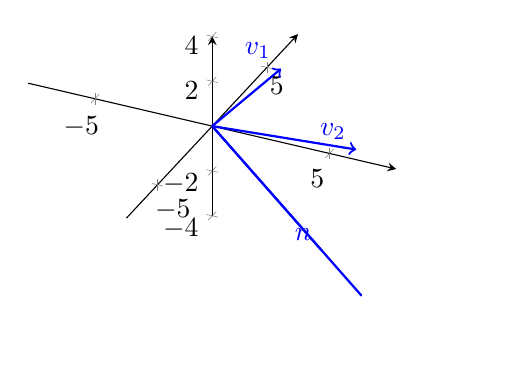
\begin{tikzpicture}
\begin{axis}[axis lines=middle, xmin=-3, xmax=3, ymin=-3,ymax=3, zmin=-4, zmax=4,axis equal,grid=both]
\addplot3 [->, thick,  blue] coordinates { (0,0,0) (2,2,2)}node[above left]{$v_1$};
\addplot3 [->, thick,  blue] coordinates { (0,0,0) (8,-4,3)}node[above left]{$v_2$};
\addplot3 [->, thick,  blue] coordinates { (0,0,0) (14,10,-24)}node[below]{$n$};
\addplot3 [thick,  blue] coordinates { (0,0,0) (3.5,2.5,-6)}node[above left]{$n$};
\end{axis}
\end{tikzpicture}

\section{Dot product}
Solve for the angle between $v_1 \text{ and } v_2$\\
$v_1=\begin{bmatrix}
1  \\
-2   \\
3
\end{bmatrix}
v_2=\begin{bmatrix}
4  \\
0   \\
1
\end{bmatrix}$\\\\
\textbf{Solution: }
$ arccos(\frac{v_1 \cdot v_2}{|v_1| |v_2}|)=arccos(\frac{\begin{bmatrix}
1\\
-2\\
3
\end{bmatrix} \cdot \begin{bmatrix}
4\\
0\\
1
\end{bmatrix}}{|\begin{bmatrix}
1\\
-2\\
3
\end{bmatrix}| |\begin{bmatrix}
4\\
0\\
1
\end{bmatrix}|})=arccos(\frac{1*4+-2*0+3*1}{\sqrt{1^2+-2^2+3^2}\sqrt{4^2+0^2+1^2}})=arccos(\frac{7}{\sqrt{14}\sqrt{17}})=arccos(.45)=63.26^\circ$

\section{Frames, translations and rotations}
Given frames: Frame \{A\} = universe,\\ 
Frame \{B\} = \{${}^{A}_{B}R=\begin{bmatrix}
cos(135) & -sin(135) \\
sin(135) & cos(135)
\end{bmatrix} ,{}^{A}P_{Borg}=\begin{bmatrix}
3  \\
4 
\end{bmatrix} $\},\\
Frame \{C\} = \{${}^{B}_{C}R=\begin{bmatrix}
cos(-30) & -sin(-30) \\
sin(-30) & cos(-30)
\end{bmatrix} ,{}^{B}P_{Corg}=\begin{bmatrix}
-2  \\
2 
\end{bmatrix} $\},\\
Frame \{D\} = \{${}^{A}_{D}R=\begin{bmatrix}
cos(0) & -sin(0) \\
sin(0) & cos(0)
\end{bmatrix} ,{}^{A}P_{Dorg}=\begin{bmatrix}
3  \\
-3 
\end{bmatrix} $\},\\
Frame \{E\} = \{${}^{A}_{E}R=\begin{bmatrix}
cos(60) & -sin(60) \\
sin(60) & cos(60)
\end{bmatrix} ,{}^{A}P_{Eorg}=\begin{bmatrix}
0  \\
0 
\end{bmatrix} $\},\\
Frame \{F\} = \{${}^{A}_{F}R=\begin{bmatrix}
cos(45) & -sin(45) \\
sin(45) & cos(45)
\end{bmatrix} ,{}^{A}P_{Forg}=\begin{bmatrix}
-1  \\
-1 
\end{bmatrix} $\},\\
Frame \{G\} = \{${}^{F}_{G}R=\begin{bmatrix}
cos(90) & -sin(90) \\
sin(90) & cos(90)
\end{bmatrix} ,{}^{F}P_{Gorg}=\begin{bmatrix}
-2  \\
5 
\end{bmatrix} $\}\\\\
Given points: ${}^{A}P_{1}=\begin{bmatrix}
3  \\
-2 
\end{bmatrix}$, ${}^{B}P_{2}=\begin{bmatrix}
8  \\
6 
\end{bmatrix}$, ${}^{C}P_{3}=\begin{bmatrix}
-3  \\
-5 
\end{bmatrix}$, ${}^{D}P_{4}=\begin{bmatrix}
-2  \\
4 
\end{bmatrix}$,${}^{E}P_{5}=\begin{bmatrix}
.7  \\
.7 
\end{bmatrix}$, ${}^{F}P_{6}=\begin{bmatrix}
-3.14  \\
2.718 
\end{bmatrix}$, ${}^{G}P_{7}=\begin{bmatrix}
3  \\
4 
\end{bmatrix}$ \\\\\\
Questions:\\
1. Draw the frames and points given above.\\
2. Compute ${}^{A}_{C}T$ and ${}^{A}_{G}T$. \\
3. Find ${}^{D}P_{1}$ and ${}^{A}P_{4}$. \\
4. Find ${}^{E}P_{1}$ and ${}^{A}P_{5}$. \\
5. Find ${}^{B}P_{1}$ and ${}^{A}P_{2}$.\\
6. Find ${}^{F}P_{1}$ and ${}^{A}P_{6}$. \\
7. Find ${}^{F}P_{2}$ and ${}^{B}P_{6}$. \\
8. Find ${}^{D}P_{5}$ and ${}^{E}P_{4}$. \\
9. Find ${}^{C}P_{7}$ and ${}^{G}P_{3}$. \\
A. Apply a rotation of $-80^\circ$ and translate by vector $v=\begin{bmatrix}
-6  \\
7 
\end{bmatrix}$ to ${}^{A}P_{1}$.\\
B. Apply a rotation of $130^\circ$ and translate by vector $v=\begin{bmatrix}
4  \\
-2 
\end{bmatrix}$ to ${}^{C}P_{7}$.\\\\
\textbf{Solution: }
\textbf{1. }\\
\begin{tikzpicture}[scale=2]
\begin{axis}[axis lines=middle, xmin=-10, xmax=10, ymin=-10,ymax=10,axis equal,grid=both]
\addplot [black] coordinates { (0,0) (0,0)}node[below]{$\{A\}$};
\addplot [->, thick,  red] coordinates { (0,0) (3,-2)}node[below]{$\mathbf{^A P_1}$};

\addplot [->, thick,  black] coordinates { (3,4) (2.29,4.71)}node[above left];
\addplot [->, thick,  black] coordinates { (3,4) (2.29,3.29)}node[above left];
\addplot [black] coordinates { (3,4) (3,4)}node[below]{$\{B\}$};
\addplot [->, thick,  red] coordinates { (3,4) (-6.9,3.41)}node[above left]{$\mathbf{^B P_2}$};

\addplot [->, thick,  black] coordinates { (3,1.17) (2.74,2.14)}node[above left];
\addplot [->, thick,  black] coordinates { (3,1.17) (2.03,.91)}node[above left];
\addplot [black] coordinates { (3,1.17) (3,1.17)}node[below]{$\{C\}$};
\addplot [->, thick,  red] coordinates { (3,1.17) (8.6,-.43)}node[above left]{$\mathbf{^C P_3}$};

\addplot [->, thick,  black] coordinates { (3,-3) (4,-3)}node[above left];
\addplot [->, thick,  black] coordinates { (3,-3) (3,-2)}node[above left];
\addplot [black] coordinates { (3,-3) (3,-3)}node[below]{$\{D\}$};
\addplot [->, thick,  red] coordinates { (3,-3) (1,1)}node[above]{$\mathbf{^D P_4}$};

\addplot [->, thick,  black] coordinates { (0,0) (.5,.87)}node[above left];
\addplot [->, thick,  black] coordinates { (0,0) (-.87,.5)}node[above left];
\addplot [black] coordinates { (0,0) (0,0)}node[left]{$\{E\}$};
\addplot [->, thick,  red] coordinates { (0,0) (-.26,.96)}node[above]{$\mathbf{^E P_5}$};

\addplot [->, thick,  black] coordinates { (-1,-1) (-.29,-.29)}node[above left];
\addplot [->, thick,  black] coordinates { (-1,-1) (-1.71,-.29)}node[above left];
\addplot [black] coordinates { (-1,-1) (-1,-1)}node[left]{$\{F\}$};
\addplot [->, thick,  red] coordinates { (-1,-1) (-5.14,-1.3)}node[above]{$\mathbf{^F P_6}$};

\addplot [->, thick,  black] coordinates { (-5.9,1.12) (-6.65,1.83)}node[above left];
\addplot [->, thick,  black] coordinates { (-5.9,1.12) (-6.65,.41)}node[above left];
\addplot [black] coordinates { (-5.9,1.12) (-5.9,1.12)}node[left]{$\{G\}$};
\addplot [->, thick,  red] coordinates { (-5.9,1.12) (-10.9,.41)}node[above]{$\mathbf{^G P_7}$};
\end{axis}
\end{tikzpicture}\\\\
\textbf{2. } ${}^A_CT={}^A_BT{}^B_CT=\begin{bmatrix}
c135 & -s135 & 3 \\
s135 & c135 & 4 \\
0 & 0 & 1
\end{bmatrix}\begin{bmatrix}
c-30 & -s-30 & -2 \\
s-30 & c-30 & 2 \\
0 & 0 & 1
\end{bmatrix}=\begin{bmatrix}
-.26 & -.97 & 3 \\
.97 & -.26 & 1.17 \\
0 & 0 & 1
\end{bmatrix}$\\\\
${}^A_GT={}^A_FT{}^F_GT=\begin{bmatrix}
c45 & -s45 & -1 \\
s45 & c45 & -1 \\
0 & 0 & 1
\end{bmatrix}\begin{bmatrix}
c90 & -s90 & -2 \\
s90 & c90 & 5 \\
0 & 0 & 1
\end{bmatrix}=\begin{bmatrix}
-.71 & -.71 & -5.95 \\
.71 & -.71 & 1.12 \\
0 & 0 & 1
\end{bmatrix}$\\\\
\textbf{3. } ${}^DP_1={}^D_AT{}^AP_1=\begin{bmatrix}
1 & 0 & -3\\
0 & 1 & 3\\
0 & 0 & 1
\end{bmatrix}\begin{bmatrix}
3\\
-2\\
1
\end{bmatrix}=\begin{bmatrix}
0\\
1\\
1
\end{bmatrix}$\\\\
${}^AP_4={}^A_DT{}^DP_4=\begin{bmatrix}
1 & 0 & 3\\
0 & 1 & -3\\
0 & 0 & 1
\end{bmatrix}\begin{bmatrix}
-2\\
4\\
1
\end{bmatrix}=\begin{bmatrix}
1\\
1\\
1
\end{bmatrix}$\\\\
\textbf{4. }
${}^EP_1={}^E_AT{}^AP_1=\begin{bmatrix}
.5 & .87 & 0\\
-.87 & .5 & 0\\
0 & 0 & 1
\end{bmatrix}\begin{bmatrix}
3\\
-2\\
1
\end{bmatrix}=\begin{bmatrix}
-.23\\
-3.6\\
1
\end{bmatrix}$\\\\
${}^AP_5={}^A_ET{}^EP_5=\begin{bmatrix}
.5 & -.87 & 0\\
.87 & .5 & 0\\
0 & 0 & 1
\end{bmatrix}\begin{bmatrix}
.7\\
.7\\
1
\end{bmatrix}=\begin{bmatrix}
-.26\\
.96\\
1
\end{bmatrix}$\\\\
\textbf{5. }
${}^BP_1={}^B_AT{}^AP_1=\begin{bmatrix}
-.71 & .71 & -.71\\
-.71 & -.71 & 4.95\\
0 & 0 & 1
\end{bmatrix}\begin{bmatrix}
3\\
-2\\
1
\end{bmatrix}=\begin{bmatrix}
-4.24\\
4.24\\
1
\end{bmatrix}$\\\\
${}^AP_2={}^A_BT{}^BP_2=\begin{bmatrix}
c135 & .-s135 & 3\\
s135 & c135 & 4\\
0 & 0 & 1
\end{bmatrix}\begin{bmatrix}
8\\
6\\
1
\end{bmatrix}=\begin{bmatrix}
-6.9\\
3.41\\
1
\end{bmatrix}$\\\\
\textbf{6. }
${}^FP_1={}^F_AT{}^AP_1=\begin{bmatrix}
.71 & .71 & 1.41\\
-.71 & .71 & 0\\
0 & 0 & 1
\end{bmatrix}\begin{bmatrix}
3\\
-2\\
1
\end{bmatrix}=\begin{bmatrix}
2.12\\
-3.54\\
1
\end{bmatrix}\\\\
{}^AP_6={}^A_FT{}^FP_6=\begin{bmatrix}
.71 & -.71 & -1\\
.71 & .71 & -1\\
0 & 0 & 1
\end{bmatrix}\begin{bmatrix}
-3.14\\
2.718\\
1
\end{bmatrix}=\begin{bmatrix}
-5.14\\
-1.29\\
1
\end{bmatrix}$\\\\
\textbf{7. }
${}^FP_2={}^F_AT{}^AP_2=\begin{bmatrix}
.71 & .71 & 1.41\\
-.71 & .71 & 0\\
0 & 0 & 1
\end{bmatrix}\begin{bmatrix}
-6.9\\
5.41\\
1
\end{bmatrix}=\begin{bmatrix}
.36\\
8.71\\
1
\end{bmatrix}\\\\
{}^BP_6={}^B_AT{}^AP_6=\begin{bmatrix}
-.71 & .71 & -.71\\
-.71 & -.71 & 4.95\\
0 & 0 & 1
\end{bmatrix}\begin{bmatrix}
-5.14\\
-1.29\\
1
\end{bmatrix}=\begin{bmatrix}
2.01\\
9.5\\
1
\end{bmatrix}$\\\\
\textbf{8. }
${}^DP_5={}^D_AT{}^AP_5=\begin{bmatrix}
1 & 0 & -3\\
0 & 1 & 3\\
0 & 0 & 1
\end{bmatrix}\begin{bmatrix}
-.26\\
.96\\
1
\end{bmatrix}=\begin{bmatrix}
-3.26\\
3.96\\
1
\end{bmatrix}\\\\
{}^EP_4={}^E_AT{}^AP_4=\begin{bmatrix}
.5 & .87 & 0\\
-.87 & .5 & 0\\
0 & 0 & 1
\end{bmatrix}\begin{bmatrix}
1\\
1\\
1
\end{bmatrix}=\begin{bmatrix}
1.37\\
-.37\\
1
\end{bmatrix}$\\\\
\textbf{9. }
${}^CP_7={}^C_AT{}^A_GT{}^AP_1=\begin{bmatrix}
-.26 & .97 & -.36\\
-.97 & -.26 & 3.2\\
0 & 0 & 1
\end{bmatrix}\begin{bmatrix}
-.71 & -.71 & -3.95\\
.71 & -.71 & 1.12\\
0 & 0 & 1
\end{bmatrix}
\begin{bmatrix}
3\\
4\\
1
\end{bmatrix}=\begin{bmatrix}
2.87\\
13.62\\
1
\end{bmatrix}\\\\
{}^GP_3={}^G_AT{}^A_CT{}^CP_3=\begin{bmatrix}
-.71 & .71 & -5\\
-.71 & -.71 & -3.41\\
0 & 0 & 1
\end{bmatrix}
\begin{bmatrix}
-.26 & -.97 & 3\\
.97 & -.26 & 1.17\\
0 & 0 & 1
\end{bmatrix}
\begin{bmatrix}
-3\\
-5\\
1
\end{bmatrix}=\begin{bmatrix}
-6.39\\
-12.19\\
1
\end{bmatrix}$\\\\
\textbf{A. }
$T=\begin{bmatrix}
c-80 & -s-80 & -6\\
s-80 & c-80 & 7\\
0 & 0 & 1
\end{bmatrix}$\\\\
$^AP'_1=T{}^AP_1=\begin{bmatrix}
c-80 & -s-80 & -6\\
s-80 & c-80 & 7\\
0 & 0 & 1
\end{bmatrix}\begin{bmatrix}
3\\
-2\\
1
\end{bmatrix}=\begin{bmatrix}
-7.45\\
3.7\\
1
\end{bmatrix}$\\\\
\textbf{B. }
$T=\begin{bmatrix}
c130 & -s130 & 4\\
s130 & c130 & -2\\
0 & 0 & 1
\end{bmatrix}$\\\\
$^CP'_7=T{}^CP_7=\begin{bmatrix}
c130 & -s130 & 4\\
s130 & c130 & -2\\
0 & 0 & 1
\end{bmatrix}\begin{bmatrix}
2.87\\
13.62\\
1
\end{bmatrix}=\begin{bmatrix}
-8.28\\
-8.56\\
1
\end{bmatrix}$

\section{Programming question 1}
In python use numpy, opencv, or code your own functions to verify your answers are correct for parts 1-6.
Or you can use c++ with \\eigen(https://eigen.tuxfamily.org/index.php?title=Main\_Page) or install opencv in c++, to verify your answers for parts 1-6. \textbf{Submit as .py or .cpp file. I should be able to run your code and get the answers for parts 1-6.}\\\\
\textbf{CODE ON BLACKBOARD}

\section{Programming question 2}
Create a class in python or c++ to represent a 2D frame object. Make sure to include at least parent frame, child frame, origin, and orientation.\\
\textbf{1. } Write a function for multiplying frames. This should return a new frame object.\\\\
\textbf{2. } Write a function that takes as input a point, rotation, and translation, then returns a new point that has been rotated and translated.\\\\
\textbf{3. } Write a function that takes from\_frame, to\_frame, and a point in from\_frame as input, and returns the point in to\_frame.\\\\
\textbf{4. }  Use your class to verify your answers from part 7.\\
\textbf{submit the .py or .cpp files you created}\\\\
\textbf{CODE ON BLACKBOARD}

\end{document}
